\section{Experiments}
In this section, we will introduce the datasets we construct from multiple business lines, and discuss our experimental results under single-domain \& multi-domain product categorization scenarios. We further discuss the generalizability of \textit{TaLR} under zero-shot conditions (evolving taxonomy  \& new taxonomy). A brief comparison of time efficiency between \textit{TaLR} and simple \textit{Reranking} is also included. 

\subsection{Dataset Analysis}
To address the multi-domain taxonomies challenge, we select 3 business lines from our e-commerce platform: 
QuickDelivery (QD, targeting fast delivery), BargainHunters (BH, targeting low price), FreshGrocery (FG, targeting fresh vegetables). 
These data instances 
% including product titles and category labels 
are collected from the real-world business, where the product titles are mostly assigned by sellers from the platform and the category labels stem from pre-defined business taxonomies. Both product titles and category labels are in Chinese. We recruit experienced annotators to manually classify the products into assorted categories, with 1\% sampling to verify the annotation accuracy. Data groups with over 95\% accuracy in sample quality checking are used in our final datasets. 
Examples in \tabref{tb:exa} are translated from Chinese.

\begin{table}[th]
\begin{threeparttable}[b]
  \caption{Dataset statistics from multiple business lines}
  \label{tb:dataset}
  \centering
  \begin{tabular}{l|ccccc}
    \toprule
    Dataset & \#training  & \#test  & \#classes & depth  & evolve \\
    \midrule
    \small{QuickDelivery} & 99k & 11k & 1987 & 3 & yes  \\
    \small{BargainHunters} & 31k & 5k & 2632 & 4 & no \\
    \small{FreshGrocery} & 28k & 3k & 1065 & 4 & no \\
    \bottomrule
  \end{tabular}
  \begin{tablenotes}
    \item[1] \#classes: the total distinct leaf node categories in each taxonomy.
    \item[2] depth: the category taxonomy tree depth.
  \end{tablenotes}
  \end{threeparttable}
\end{table}

\begin{table}[th]
  % \setlength{\tabcolsep}{2.5pt}
  \caption{Examples from the three Datasets}
  \label{tb:exa}
  \centering
  \begin{tabular}{c|c|c}
    \toprule
     Data & Product title  & Taxonomy path \\
     \midrule
     QD & \tabincell{c}{\textit{Towel gourd 1 pcs} \\ \textit{\& soy bean 150g}} & \tabincell{c}{\small{Vegetable} $\rightarrow$ \small{Mixed Product} \\ $\rightarrow$  \small{Vegetables mixture}}\\
     \midrule
     BH & \tabincell{c}{\textit{Fresh bamboo shoots} \\ \textit{(dig from mountains)}} & \tabincell{c}{\small{Vegetable/Fruit} $\rightarrow$ \small{Vegetable} \\$\rightarrow$ \small{Tubers} $\rightarrow$ \small{Bamboo}}\\
     \midrule
     FG & \tabincell{c}{\textit{Butter leaf lettuce 100g}} & \tabincell{c}{\small{Fresh} $\rightarrow$ \small{Vegetable} $\rightarrow$ \\ \small{Leaf} $\rightarrow$ \small{Lettuce}}\\
    \bottomrule
  \end{tabular}
\end{table}

Statistics of 
% these 3 product categorization 
three datasets are listed in \tabref{tb:dataset}. The number of classes reveals the large scale of classes in each taxonomy, and different taxonomy trees may 
% have different 
vary in
depths, which poses a bigger challenge for multi-domain knowledge sharing. 

To test the generalizability of \textit{TaLR} on the evolving taxonomy  challenge, We further construct two taxonomy evolving derivatives of QD test set. 
(ii) QD-$integrate$: 
% the original category nodes are renamed into new ones. There are 1371 samples in this subset, with 127 classes before and \TODO{127} classes after renaming.
During a production business adjustment, 127 classes in the original taxonomy are integrated or replaced by similar categories, which affects 1371 samples in the original test set to form this subset. Products map their original categories with integrated ones.
(i) QD-$divide$: 
22 category nodes from the original QD taxonomy are divided into two or more nodes.
% to simulate the deletion of old nodes and increment of new nodes. 
This subset is comprised of 495 samples in the test set which suffer from this evolution, and we assign them with suitable new categories within divided ones using some heuristics. 
\subsection{Baselines}
\label{sec: baseline}
% \TODO{Intro: TF-IDF+LR, fastText, BERT, multi-task,...}
We implement several baseline methods based on single-domain, multi-domain and zero-shot scenarios.
\subsubsection{Single-domain}
For methods targeting the single domain categorization task, we train individual models for each domain.

\noindent \textbf{TF-IDF\&LR} represents product titles with TF-IDF weighted dense vectors, and executes classification with Logistic Regression.

\noindent \textbf{fastText} \cite{bojanowski2017enriching} is a common baseline adopted in online product categorization challenges. It leverages bag-of-words features and subword information for text classification.

\noindent \textbf{BERT} \cite{devlin-etal-2019-bert} represents the generic BERT text classification approach with encoded [$\mathtt{CLS}$] token and a fully-connected layer followed by softmax function.
\subsubsection{Multi-domain}
We exploit \textbf{multi-task} learning paradigm as strong baseline for multi-domain categorization. A shared BERT is utilized as the text encoder with multiple output heads targeting different tasks. Data batches from each task take turns to update the model weightings during training, where the loss function is formulated by summing up multi-class cross entropy losses across different tasks.
\subsubsection{Zero-shot Setting}
Since all the above baselines cannot tackle with zero-shot conditions (evolving taxonomy  \& new taxonomy) without re-training, we instead utilize separate BERT classifiers trained with few-shot data (1\%) on each task respectively as a strong baseline \textbf{BERT-few-shot}. 
% For zero-shot conditions (evolving taxonomy  \& new taxonomy), 
In addition, we adopt the vanilla BERT without training to encode both product titles and category names and calculate their semantic similarity with [$\mathtt{CLS}$] token as a weaker baseline \textbf{BERT-matching}. 
While each component of \textit{TaLR} could be used individually under zero-shot scenarios, the ablations of \textit{TaLR} can also be regarded as competitive zero-shot alternatives. 
% For zero-shot conditions (evolving taxonomy  \& new taxonomy), we adopt the BERT continually pretrained with Masked Language Modeling on ? product titles from heterogeneous business scenarios, denoted as \textbf{BERT-product}. We encode product titles and category labels respectively with BERT-product represented by [$\mathtt{CLS}$] tokens. Predicted category label is the top-1 candidate during on-vs-all similarity comparison between encoded product title $X$ and all category labels in evolved taxonomy. 
\subsection{Experimental Setup}
\subsubsection{Implementation Details}
\label{sec:exp detail}
For fair comparisons, we deploy all experiments on 48 core Intel(R) Xeon(R) CPU E5-2650 v4 @ 2.20GHz and Nvidia Geforce A100 80G GPU.
All the ``BERT'' abbreviations mentioned in this work are Google BERT-base pretrained on Chinese corpus. 
For TF-IDF and fastText baselines, We use jieba\footnote{\href{https://github.com/fxsjy/jieba}{https://github.com/fxsjy/jieba}} toolkit to generate Chinese word segments and tune hyper-parameters on each dataset respectively. 
Baselines like BERT-classifier, k-fold generator and bi-encoder BERT in vector-based retrieval are trained with 2e-5 learning rate, 512 batch size, 32 sequence length, and maximum 40 epochs.
% with early stopping patience set to 3
Multi-task baseline adopts the same settings and adds up three losses with equal weights. Cross-encoder BERT classifier in \textit{Reranking} stage extends sequence length to 64 catering for the concatenation of $X$ and $y$ while other settings remain. 

In the vector-based retrieval stage, we use Annoy\footnote{\href{https://github.com/spotify/annoy}{https://github.com/spotify/annoy}} toolkit to effectively search for embeddings in category label space that are close to a given product embedding vector. Considering the run-time trade-off between better accuracy and speed, we set the number of indexing trees to be 20000.

We mix up training data from three datasets to train the unified \textit{TaLR}. 
% We also experimented the performance of \textit{TaLR} trained on each dataset separately. 
% \TODO{TaLR training and different inference strategies on different dataset}
During training and testing, the rule-based unit is used concurrently with the vector-based unit under ordinary product categorization or multi-domain scenarios. However, it is disabled when zero-shot challenges (evolving taxonomy  \& new taxonomy) are encountered in that incoming new categories are invisible in original training set distributions. Thus in such scenarios, the rule-based unit is used only in the training procedure, so we can not ablate the vector-based unit during zero-shot inference.
\subsubsection{Evaluation Metrics}
In \textit{Retrieval} stage, we use widely-used metrics \textbf{HR}@$k$ (Hit Rate) to measure the capacity of models to retrieve the correct categories, where $k$ could be $1,10$. For the whole framework, we use \textbf{accuracy} score as the classification metric. TP, TN, FN, FP refer to the true positive, true negative, false negative and false positive predictions respectively, and accuracy is calculated by $\frac{TP}{TP+TN+FN+FP}$, which mathematically equals to \textbf{Micro-F1} score in single-label multi-class classification problem. \textbf{Micro-F1} is the F1-score averaged over all instances. 

\subsection{Overall Results}
\label{sec:all res}
The overall accuracy score is shown in \tabref{tb:all}, and we can make the following observations.

\begin{table}[!th]
\setlength{\tabcolsep}{4pt}
  \begin{threeparttable}[b]
  \caption{The accuracy of our \textit{TaLR} framework on three business lines with many variants of \textit{TaLR}. The best results are bolded, and the wavy-underlined results refer to the most drop in ablation test.}
  \label{tb:all}
  \centering
  \begin{tabular}{l|cccc}
    \toprule
    Methods & Overall & QD & BH & FG\\
    \midrule
    \multicolumn{5}{c}{Separate models}\\
    \midrule
    TF-IDF-classifier $^{\ddagger}$ & 69.51 & 69.93 & 68.23 & 69.95 \\
    fastText-classifier $^{\ddagger}$ & 74.62 & 74.01 & 71.68 & 80.82 \\
    BERT-classifier $^{\ddagger}$ & 83.49 & 84.82 & 79.93 & 84.23\\
    % HFGN-F-classifier $^{\ddagger}$ & - & 83.72 & 77.09 & 84.25 \\
    \textit{TaLR} $^{\ddagger}$ & 85.90 & 87.88 & 81.92 & 85.09\\
    \midrule
    \multicolumn{5}{c}{Unified model}\\
    \midrule
    BERT Multi-task & 64.41 & 76.79 & 50.26 & 44.09 \\
    \textit{TaLR} & \textbf{86.23} & \textbf{88.16} & \textbf{82.48} & \textbf{85.25}\\
    \midrule
    \multicolumn{5}{c}{\textit{TaLR} ablation test}\\
    \midrule
    (-) rerank stage \tiny{[bi-encoder]} & \uwave{82.29} $\downarrow$ & 84.19 $\downarrow$ & \uwave{77.63} $\downarrow$ & 82.72 $\downarrow$\\
    (-) retrieval stage \tiny{[cross-encoder]} & 83.29 $\downarrow$ & 84.95 $\downarrow$ & 80.53 $\downarrow$ & \uwave{81.78} $\downarrow$\\
    \midrule
    (-) contrastive learnig & 85.26 $\downarrow$ & 86.83 $\downarrow$ & 81.75 $\downarrow$ & 85.13 $\downarrow$\\
    (-) rule-based unit & 82.82 $\downarrow$ & \uwave{83.85} $\downarrow$ & 79.15 $\downarrow$ & 84.71 $\downarrow$\\
    (-) vector-based unit & 84.91 $\downarrow$ & 86.52 $\downarrow$ & 81.66 $\downarrow$ & 84.28  $\downarrow$\\
    \bottomrule
  \end{tabular}
  \begin{tablenotes}
    \item[1] The overall accuracy is measured on the test data with 3 business lines combined, and we list separate accuracy on each subset.
    \item[2] Methods with $^{\ddagger}$ notation train three separate models on the three datasets of business lines and infer using its corresponding model. Methods without $^{\ddagger}$ only train one unified model using multi-domain data.
    \item[3] (-) denotes the ablation of following modules in our framework.
  \end{tablenotes}
  \end{threeparttable}
\end{table}

Under traditional product categorization conditions, we train separate models on each dataset respectively. 
Among methods targeting one static taxonomy, the BERT-classifier performs better than LR model based on the TF-IDF feature and fastText model, indicating the good generalization ability of BERT aided with pretrained knowledge. 
However, because these methods can only handle one static taxonomy for each business line, they not only suffer from efforts to maintain different models but also fail to leverage multi-domain data. 
The multi-task method is able to train and infer three tasks within one model to solve the multi-domain challenge, but it performs even worse than TF-IDF. 
One possible reason is that the multi-task approach relies heavily on the generality of tasks, and if the task-specific training data distribution varies significantly, one easiest task might govern the joint distribution and constrain the optimization of other tasks.
% heavily relies on the appropriate choice of weighting between each task’s loss, but the naive weights is hard to manually tuned and might easily impact the learning procedure. 
% The accuracy on QD is the highest and on BH is the lowest since the number of training samples on QD is the most whereas the number of classes on BH is the most, intensifying the difficulty to classify.


For our proposed framework \textit{TaLR}, it not only outperforms other baselines in separate model training paradigm but achieves even higher accuracy on the more complicated multi-domain challenge which simple multi-task learning fails to support,
% it outperforms multi-task learning method and 
% other separately trained classifiers, 
showing its capacity to tackle \textbf{multi-domain taxonomies} challenge. 
% We also deploy \textit{TaLR} in separately-training manner, as shown, \textit{TaLR} is slightly better than \textit{TaLR} $^{\ddagger}$. 
As is shown in \tabref{tb:all}, the unified \textit{TaLR} is slightly better than \textit{TaLR} $^{\ddagger}$, which
verifies our cross-domain knowledge sharing assumption. Note that the products and category names from multiple taxonomies are not absolutely different from each other (see \tabref{tb:exa}), instead they may share similar semantic meanings, which promotes the performance on the overall multi-domain dataset as well as on each respective business. Furthermore, given BERT-classifier as the baseline, we compare \textit{TaLR} after removing the \textit{Reranking} stage, which is the BERT bi-encoder, and \textit{TaLR} after removing the \textit{Retrieval} stage, which is the BERT cross-encoder, and the results is less or close to the baseline. This result further corroborates that the improvement of \textit{TaLR} from \textit{TaLR} $^{\ddagger}$ is contributed by the knowledge integration capability of the framework instead of purely addition of data.

From the ablation test, we can show the effects of different units in our \textit{TaLR} framework. 
Removing \textit{Rerank} stage drops the overall accuracy most, and within this stage, contrastive learning plays a significant role, showing the power of our cross-encoder with contrastive information to semantically align the embeddings of product titles and category names from multiple domains. Removing the rule-based unit impairs the overall results mainly on account of the external knowledge imported from the meta label set. Considering that the rule-based unit establishes a mapping from meta labels to categories through training set distribution, 
% the meta label set is stem from training set, 
it will be disabled when taxonomy evolving or even new taxonomies are encountered. In that situation, the vector-based unit will take over to support zero-shot instances, although it is less effective in this ablation test.

\subsection{Time Consumption}
\label{sec:time cons}
A big concern of our framework is to limit the run-time overheads, since the large label space challenge may deteriorate in one-vs-all retrieval systems rather than classification approaches.  
Thus we compare the inference speed (seconds cost for each instance) of \textit{TaLR} with the single BERT cross-encoder model that we train and test on our three standard datasets. Here the single BERT cross-encoder computes the similarity score over all category classes and selects the most similar one as the prediction, while \textit{TaLR} instead utilized bi-encoder with cached category embeddings to conduct one-vs-all retrieval and the cross-encoder BERT in \textit{Reranking} stage takes only 10 candidates. 
\figref{fig:time} plots the relationship between the number of classes and the inference speed. On the one hand, the inference speed of \textit{TaLR} is much faster (4 times faster for FG and 10 times faster for BH) than BERT cross-encoder owing to the \textit{Retrieval} stage. On the other hand, the time consumption per item of \textit{TaLR} increases almost linearly along with the number of classes, while for BERT cross-encoder the overhead grows more sharply, revealing the time efficiency of \textit{TaLR} when the class number scales. 
% As for the accuracy score, \textit{TaLR} fluctuates in the same pace with BERT cross-encoder but consistently outperforms it, and the reason of fluctuation is explained before.
\textit{TaLR} also consistently outperforms single BERT cross-encoder in accuracy due to the selection of better candidates in \textit{Retrieval} stage. 

\begin{figure}[thbp] \centering
    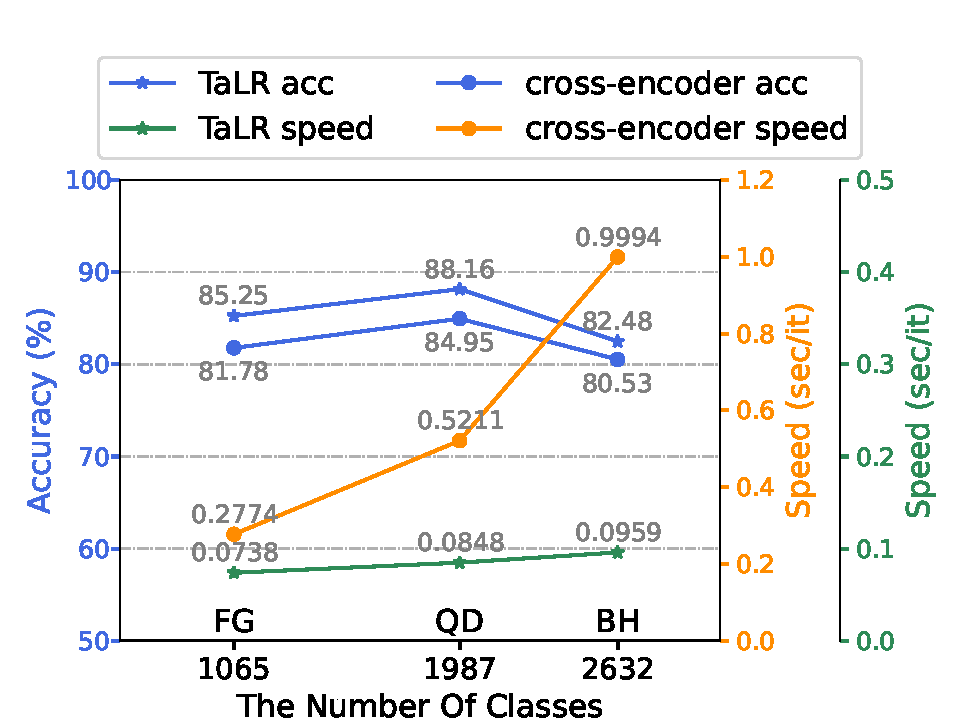
\includegraphics[width=0.38\textwidth]{time.pdf}
    \caption{Inference speed and accuracy results as the number of classes goes on.} 
    \label{fig:time}
\end{figure}

\subsection{Evolving Taxonomy Experiment}
\label{sec:evolve res}
In order to evaluate the ability of our framework on \textbf{evolving taxonomy} challenge, 
we use \textit{TaLR} trained on multi-domain datasets to directly infer product titles on evolved taxonomies.
% we directly infer product titles with \textit{TaLR} trained on multi-domain datasets on the evolved taxonomies.
% we conduct experiments to directly infer evolved new category of the product with \textit{TaLR}. 
Here ``before'' denotes the subset from original test set, while ``after'' denotes the subset with the same product titles but evolved categories.
From the listed accuracy ``before'' and ``after'' taxonomy evolving in \figref{tb:evolve}, we can conclude that \textit{TaLR} sustains accuracy within a tolerable range.
% the encoded [$\mathtt{CLS}$] token similarity from %%% explained before
BERT-matching is the vanilla similarity matching baseline and BERT-few-shot is the separate fews-shot classifiers we mentioned in \secref{sec: baseline}. Note that BERT-few-shot could be trained on full data before evolving.


\begin{table}[th]
% \small
\setlength{\tabcolsep}{3pt}
  \begin{threeparttable}[b]
  \caption{The accuracy of \textit{TaLR} framework on two evolving taxonomy datasets. $\Delta$ is the change
  of accuracy after evolving. The best ``after'' scores and least drop $\Delta$ are bolded.}
  \label{tb:evolve}
  \centering
  \begin{tabular}{l|ccc|ccc}
    \toprule
    \multirow{2}{*}{Methods} & \multicolumn{3}{c|}{QD$-divide$} & \multicolumn{3}{c}{QD$-integrate$}\\
    \cline{2-7}
    & Before & After & $\Delta$ & Before & After & $\Delta$ \\
    \midrule
    BERT-matching & 6.66 & 11.95 & \textbf{+5.29} & 13.39 & 2.23 & -11.16\\
    BERT-few-shot & 90.51 & 43.54 & -46.96 & 86.79 & 50.16 & -36.53\\
    \midrule
    \textit{TaLR} & 90.11 & 69.71 & -20.40 & 85.20 & \textbf{81.48} & -3.72\\
    (-) contrastive  & 89.10 & \textbf{79.21} & -9.89 & 84.11 & 80.02 & -4.09\\
    (-) rerank stage & 89.70 & 73.94 & -15.76 & 86.36 & 81.47 & -4.89\\
    (-) rule-based unit & 89.51 & 64.25 & -25.26 & 84.61 & 81.19 & \textbf{-3.42}\\
    \bottomrule
  \end{tabular}
%   \begin{tablenotes}
%     \item[1] 
%   \end{tablenotes}
  \end{threeparttable}
\end{table}
On the one hand, our \textit{TaLR} even outperforms BERT-few-shot without additional training on evolved taxonomies, which indicates its strong generalizability handling dynamic issues.

On the other hand, we can observe an opposite trend of BERT-matching and \textit{TaLR} through $\Delta$ when two different evolving challenges are encountered. In node $integrate$ scenarios, \textit{TaLR} exhibits robustness with a slight drop of accuracy. 
When progressively ablating contrastive learning and the whole \textit{Reranking} stage, the accuracy of \textit{TaLR} consistently decreases, which indicates their contributions for the node \textit{integrate} derivative of evolving taxonomy.
% \textbf{Taxonomy integration}.
% On the other hand, BERT-matching suffers from a drastic drop of accuracy, which may attribute to 
However in node $divide$ scenario, wherever contrastive learning is incorporated, there is a substantial drop in $\Delta$. Completely excluding the contrastive learning while keeping all other components gives the best accuracy. 
The reason behind it is that contrastive learning tends to make the representations of products from the same category tied closer, while the division of nodes breaks this relation. So in taxonomy $divide$ situation, we strongly suggest to use \textit{TaLR} without contrastive learning.

Besides, BERT-matching suffers a cliff drop in when node $integrate$ but gains performance in node $divide$ scenario. When categories are lumped together, their meanings are often coarse-grained and vague, and thus when categories are divided into more fine-grained concepts, vanilla semantic matching methods could better capture the explicit semantic relationship between product titles and category names, and vice versa.


% In the taxonomy $integrate$ scenario, the advantage of \textit{TaLR} is more obvious, where the accuracy falls off slightly after evolving while for BERT-matching there is a cliff drop. When ablating contrastive learning, both ``after'' accuracy and $\Delta$ accuracy decline w.r.t \textit{TaLR}, suggesting that the contrastive learning benefits the robustness of framework to deal with evolving taxonomy . 
% In the taxonomy $divide$ scenario, the accuracy of BERT-matching remains low, while \textit{TaLR} without contrastive learning suffers around 10\% drop, more robust than \textit{TaLR} with contrastive learning. Here is the reason: the contrastive learning tends to make the embeddings of products from the same category tied closer, while the division of taxonomy node breaks this relation, so in this situation, we strongly suggest use \textit{TaLR} without contrastive learning.

\subsection{Extrapolating Results on New Taxonomy}
\label{sec:new tax}
% For multi-domain business lines, 
When a new business line emerges, a robust model is supposed to categorize incoming products based on the new taxonomy $G_{i+1}$. Hence it is important for \textit{TaLR} to zero-shot transfer to new taxonomies so as to improve user experience in this cold-start scenario.

We deploy our experiments in a zero-shot manner, where we take turns to train the model on either two businesses and test its performance on the test set of the remaining one. Still, our \textit{TaLR}-zero outperforms the competitive BERT-few-shot, let alone BERT-matching. 
% We compare $TaLR$ with BERT-matching model and bi-encoder BERT in zero-shot, and $TaLR$-zero sustains better accuracy, 
It is mainly because of the learning in other two datasets, which contributes to the semantic relatedness understanding in the third dataset with brand new taxonomy. Meanwhile, each component in the ablation test verifies its corresponding effectiveness. 

% More details about ablation setting is in \secref{sec:exp detail}.

\begin{table}[th]
  \begin{threeparttable}[b]
  \caption{The accuracy of \textit{TaLR} framework on the new taxonomy. }
  \label{tb:zeroshot}
  \centering
  \begin{tabular}{l|ccc}
    \toprule
    Methods & QD & BH & FG \\
    \midrule
    BERT-matching & 9.00 & 11.23 & 4.03 \\
    BERT-few-shot & 43.29 & 35.19 & 29.80 \\
    % BERT-product & 52.00 & 48.81 & 51.32 \\
    \midrule
    \textit{TaLR}-zero & \textbf{60.57} & \textbf{65.45} & \textbf{62.69}\\
    % \textit{TaLR}-few(?) &  &  & \\
    % \textit{TaLR}-finetune(?) & 84.32 & 76.40 & 83.59\\
    % \midrule
    (-) contrastive learning & 56.71 & 64.99 & 60.79\\
    (-) rerank stage \tiny{[bi-encoder]} & 53.79 & 59.56 & 57.68 \\
    (-) rule-based unit & 56.25 & 64.65 & 59.29\\
    \bottomrule
  \end{tabular}
%   \begin{tablenotes}
%     \item[1] 
%   \end{tablenotes}
  \end{threeparttable}
\end{table}

\subsection{Different Retrieval Strategies}
\label{sec:retri stra}
In \textit{Retrieval} stage, it is encouraged to exploit the potential candidates as accurately as possible, otherwise the latter \textit{Reranking} stage would never make right predictions if the true label is not covered by the retrieved candidates. Hence we use HR@$k$ to measure the retrieval performance.

Firstly, we compare several alternatives of the loss function in vector-based retrieval model. In \figref{fig:vector-retri}, as $k$ goes on, the HR score increases, and the model trained with Cosent loss is consistently better than others, while the model trained with SBERT loss performs unstably, sometimes worse than Cosine loss. 
One explanation is that comparing with Cosine loss and SBERT loss, the Cosent loss focuses on the positive-versus-negative pairwise optimization, which means the model only cares for the relative order of the prediction results instead of the specific value. And this setting brings consistent recall of candidates.
% \begin{table}[th]
%   \caption{The retrieval results of the vector-based unit over different loss function. The best results are bolded.}
%   \label{tb:vector-retrieval}
%   \centering
%   \begin{tabular}{c|c|ccc}
%     \toprule
%     Loss & Dataset & HR@1 & HR@5 & HR@10 \\
%     \midrule
%     \multirow{3}{*}{Cosine} & QD & 74.80 & 82.28 & 84.46\\
%     & BH & 72.75 & 81.77& 84.04\\
%     & FG & 65.59 & 80.40 & 83.23\\
%     \midrule
%     \multirow{3}{*}{SBERT} & QD & 82.25 & 88.96 & 90.92\\
%     & BH & 76.95 & 86.76 & 89.41\\
%     & FG & 80.67 & 87.27 & 88.86\\
%     \midrule
%     \multirow{3}{*}{Cosent} & QD & 84.19 & 88.97 & 90.30\\
%     & BH & 77.64 & 85.27 & 87.18\\
%     & FG & 82.72 & 86.66 & 87.48\\
%     \bottomrule
%   \end{tabular}
% \end{table}

\begin{figure}
  \begin{subfigure}[b]{0.49\columnwidth}
  \centering
  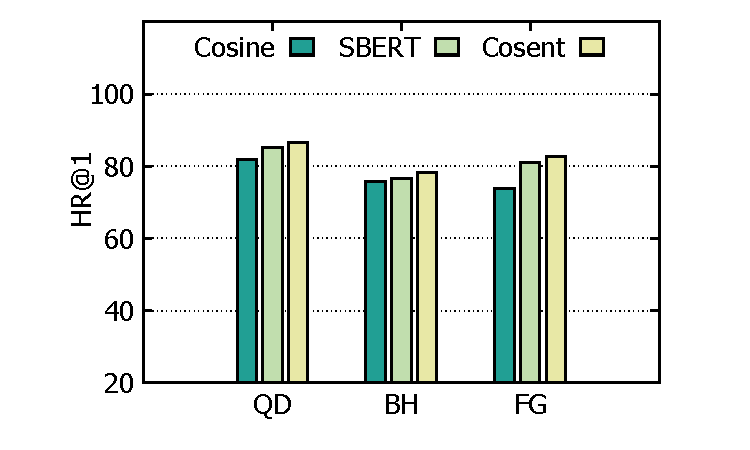
\includegraphics[width=\columnwidth]{hr_1.pdf}
  \caption{HR@1}
  \end{subfigure}
%   \hfill
%   \begin{subfigure}[b]{0.49\columnwidth}
%   \centering
%   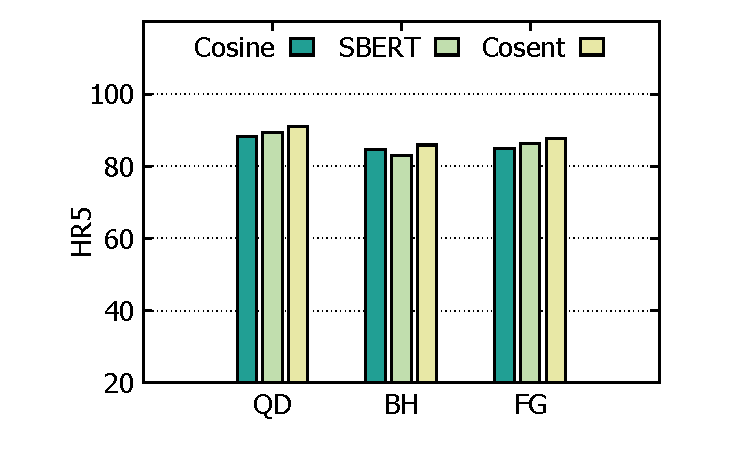
\includegraphics[width=\columnwidth]{hr_5.pdf}
%   \caption{HR@5}
%   \end{subfigure}
  \hfill
  \begin{subfigure}[b]{0.49\columnwidth}
  \centering
  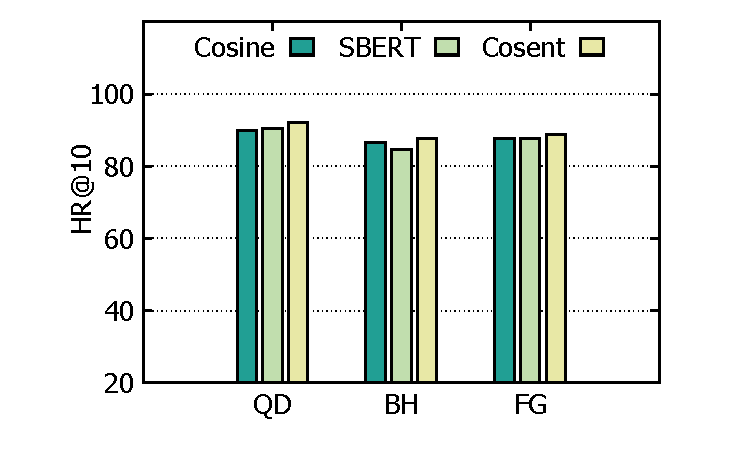
\includegraphics[width=\columnwidth]{hr_10.pdf}
  \caption{HR@10}
  \end{subfigure}
  \caption{The retrieval results of the vector-based unit over different loss functions.}
  \label{fig:vector-retri}
\end{figure}

To generate better candidates, we adopt several heuristic algorithms for two-way candidates fusion.
% the vector-based unit and rule-based unit. 
\tabref{tb:fusion} depicts the retrieval results over different fusion strategies. The size of merged candidate sets is not stick to $10$ for some of the strategies, so we list the average number.
Generally, the \textbf{Rule-First} algorithm achieves better scores, and \textbf{De-Dupli} algorithm is competitive with it. We use \textbf{Rule-First} in our framework due to its fixed candidate size which is more convenient to process.
Although the pure vector-based unit performs less effectively than the rule-based counterpart, they could complement each other after fusing together with the help of ensembled understanding of textual semantics and training set distribution.
% the ensemble of vector-based unit and rule-based unit strengthens the performance of rule-based unit, revealing that vector-based unit can better understand the instance semantically that rule-base unit can not. 
More discussions are in Case Study.

\begin{table}[th]
% \setlength{\tabcolsep}{3pt}
  \caption{The retrieval results of candidates for different fusion strategies. The best results are bolded.}
  \label{tb:fusion}
  \centering
  \begin{tabular}{c|cc|cc|cc}
    \toprule
    \multirow{2}{*}{Strategy}  & \multicolumn{2}{c|}{QD} & \multicolumn{2}{c|}{BH} & \multicolumn{2}{c}{FG} \\
    \cline{2-7} 
      & Recall & Size & Recall & Size & Recall & Size \\
    \midrule
    Rule-based & 95.33 & 8.6 & 96.77 & 8.8 & 97.32 & 9.0 \\
    Vec-based & 90.30 & 10 & 87.18 & 10 & 87.48 & 10 \\
    \midrule
    De-Dupli & 96.08 & 10.5 & \textbf{97.54} & 10.4 & 97.77 & 10.7 \\
    Norm\&Rank & 93.74 & 10 & 92.42 & 10 & 92.77 & 10 \\
    Rule-First & \textbf{96.12} & 10 & 97.48 & 10 & \textbf{98.01} & 10 \\
    \bottomrule
  \end{tabular}
\end{table}

\section{Case Study}
For product ``\textit{red dancing shoes (size 35)}'', which should be categorized to \verb|Sports/Outdoors| $\rightarrow$ \verb|Yoga/Dancing| $\rightarrow$ \verb|Dancing Shoes|, the vector-based unit retrieves the correct class as top-$1$ answer, but the rule-base unit retrieves \verb|Clothes/Shoes| $\rightarrow$ \verb|Woman Shoes| $\rightarrow$ \verb|Woman Slippers| as top-$1$. This time the distribution knowledge guides the rule-based model towards a wrong direction, while the vector-based model succeeds relying on the semantic similarity.

For product ``\textit{CHEERS$^\circledR$ 12 years}'', the vector-based model categorizes it to \verb|Books| $\rightarrow$ \verb|Economics/Management| $\rightarrow$ \verb|Marketing|, whereas the rule-based unit correctly retrieves \verb|Alcoholic Drinks| $\rightarrow$ \verb|Imported Liquors| $\rightarrow$ \verb|Whisky|. This shows that ``12 years'' misleads the vector-based model to the semantic meaning of economics, and rule-based unit successfully leverages its distribution knowledge in training set.

For product ``\textit{towel gourd\&soy bean (towel gourd 1 pcs, soy bean 150g)}'', both rule-based unit and vector-based unit predict
\verb|Vegetable| $\rightarrow$ \verb|Soy Product| $\rightarrow$ \verb|Soy Bean| wrongly as top-$1$, whereas \textit{TaLR} classifies it to correct \verb|Vegetable| $\rightarrow$ \verb|Mixed Product| $\rightarrow$ \texttt{Vegetables mixture}, and clearly, the contribution is from the following \textit{Reranking} stage.
% \begin{table*}[t]
%   \caption{The retrieval results of candidates for different fusion strategies. The best results are bolded.}
%   \label{tb:fusion}
%   \centering
%   \begin{tabular}{c|c}
%     \toprule
%     Product title & \textit{red dancing shoes (size 35)} \\
%     \midrule
%     Ground truth & \verb|Sports/Outdoors| $\rightarrow$ \verb|Yoga/Dancing| $\rightarrow$ \verb|Dancing Shoes| \\
%     Vector-based top-$1$ & \verb|Sports/Outdoors| $\rightarrow$ \verb|Yoga/Dancing| $\rightarrow$ \verb|Dancing Shoes| \\
%     Rule-based top-$1$ & \verb|Clothes/Shoes| $\rightarrow$ \verb|Woman Shoes| $\rightarrow$ \verb|Woman Slippers| \\
%     \midrule
%     Product title & \textit{CHEERS$^\circledR$ 12 years} \\
%     \midrule
%     Ground truth & \verb|Alcoholic Drinks| $\rightarrow$ \verb|Imported Liquors| $\rightarrow$ \verb|Whisky| \\
%     Vector-based top-$1$ & \verb|Books| $\rightarrow$ \verb|Economics/Management| $\rightarrow$ \verb|Marketing| \\
%     Rule-based top-$1$ & \verb|Alcoholic Drinks| $\rightarrow$ \verb|Imported Liquors| $\rightarrow$ \verb|Whisky| \\
%     \midrule
%     Product title & \textit{towel gourd \& soy bean (towel gourd 1 pcs, soy bean ~150g)} \\
%     \midrule
%     Ground truth & \verb|Vegetable&/ Product| $\rightarrow$ \verb|Mixed Product| $\rightarrow$ \verb|Vegetables mixture| \\
%     Vector-based top-$1$ & \verb|Vegetable/&Soy Product| $\rightarrow$ \verb|Soy Product| $\rightarrow$ \verb|Soy Bean| \\
%     Rule-based top-$1$ & \verb|Vegetable/Soy Product| $\rightarrow$ \verb|Soy Product| $\rightarrow$ \verb|Soy Bean| \\
%     \bottomrule
%   \end{tabular}
% \end{table*}